\documentclass[10pt,a4paper]{article}
\usepackage[margin=1.9cm]{geometry}
\usepackage{mathptmx}  % Times text and math (Type 1)
\usepackage{graphicx,booktabs,xcolor,float,tabularx,amsmath,amssymb}
\usepackage{hyperref}
\definecolor{linkblue}{RGB}{0,62,138}
\hypersetup{colorlinks=true,linkcolor=linkblue,citecolor=linkblue,urlcolor=linkblue}
\makeatletter
% section headings: "1. Title" with a normal word space, compact spacing
\renewcommand\@seccntformat[1]{\csname the#1\endcsname.\hspace{0.45em}}
\renewcommand\section{\@startsection{section}{1}{\z@}{-2.4ex \@plus -0.6ex \@minus -0.2ex}{1.0ex \@plus 0.2ex}{\normalfont\large\bfseries}}
\renewcommand\subsection{\@startsection{subsection}{2}{\z@}{-1.9ex \@plus -0.5ex \@minus -0.2ex}{0.7ex \@plus 0.2ex}{\normalfont\normalsize\bfseries}}
% captions: one size everywhere, bold label
\setlength\abovecaptionskip{5pt}\setlength\belowcaptionskip{3pt}
\long\def\@makecaption#1#2{\vskip\abovecaptionskip
  \sbox\@tempboxa{\small\textbf{#1.}\ #2}%
  \ifdim\wd\@tempboxa>\hsize {\small\textbf{#1.}\ #2\par}\else\global\@minipagefalse\hb@xt@\hsize{\hfil\box\@tempboxa\hfil}\fi
  \vskip\belowcaptionskip}
\makeatother
% every section (and the references) starts on a new page
\let\oldsection\section
\renewcommand\section{\clearpage\oldsection}
\setlength{\textfloatsep}{10pt plus 2pt minus 2pt}\setlength{\intextsep}{8pt plus 2pt minus 2pt}
\setlength{\parskip}{4pt}\setlength{\parindent}{0pt}
\graphicspath{{../Results/plots/}}
\newcommand{\code}[1]{\texttt{#1}}
\newcommand{\pp}{\,pp}
\newcommand{\best}[1]{\textbf{#1}}
\DeclareRobustCommand{\S}{\ensuremath{\mathsection}}  % Type 1 section sign, same reason
\renewcommand{\labelitemi}{$\bullet$}  % Type 1 bullet (the default \textbullet is a bitmap font in this TeX install)

\title{\vspace{-1.2cm}Multimodal Emotion Recognition on TESS:\\ speech, text and fusion pipelines\\\large Assignment 2b}
\author{Yash Tyagi\\[2pt]\small Code, results and setup instructions:\\\footnotesize\url{https://github.com/ashdev-7/iiith-fastspeech2-a2/tree/main/2b_multimodal_emotion_recognition}}
\date{November 2026}

% Hooks used when this report is included in the combined document (combined_report/); empty here.
\providecommand{\partdir}{}
\providecommand{\refshook}{}

\begin{document}
\sloppy
\maketitle
\vspace{-0.7cm}

% Assignment 2b report: the page-1 overview box (shared with combined_report/).
\begin{center}\fbox{\begin{minipage}{0.96\linewidth}\small
\textbf{At a glance} (section numbers refer to this report).\\[1pt]
\textbf{A. Architecture} (\S\ref{sec:arch}). Frozen WavLM-Base+ (speech) and emotion-tuned DistilRoBERTa (text) features feed a BiGRU with attention pooling (temporal / contextual block); a gated multimodal unit fuses the two (fusion block), and an MLP classifies.\\[2pt]
\textbf{B. Comparison} (\S\ref{sec:main}; test accuracy \%, mean over runs; chance = 14.29\%).\par\vspace{1pt}
{\centering\begin{tabular}{@{}lccc@{}}\toprule
Pipeline & Random split & Seen speakers (SD) & Unseen speaker (SI)\\\midrule
Speech (WavLM + BiGRU) & 99.86 & 99.90 & 58.48\\
Text (DistilRoBERTa + BiGRU) & 13.81 & 14.29 & 14.29\\
Fusion (gated, speech + text) & 100.00 & 99.95 & 56.77\\\bottomrule
\end{tabular}\par}\vspace{2pt}
Speech carries the emotion. Text cannot: in TESS every word is spoken in all seven emotions, so the transcript holds no information about the emotion and text alone scores exactly chance. Fusion therefore matches speech but does not beat it. The real difficulty is a new speaker: 99.9\% falls to 58.5\%.\\[2pt]
\textbf{C. Analysis} (\S\ref{sec:analysis}). Easiest emotions: neutral, sad and fear; hardest: happy and angry (\S\ref{sec:easy}). Fusion helps only where speech is uncertain and the text comes from Whisper, whose punctuation carries prosody (+5.7\pp{} net, \S\ref{sec:whenfusion}). Five failure cases (\S\ref{sec:errors}). Separability of all three blocks (Fig.~\ref{fig:tsne}, \S\ref{sec:separability}).\\[2pt]
\textbf{Beyond the brief} (\S\ref{sec:prereg}--\ref{sec:final}). Five studies, each planned and committed before it was run, raise unseen-speaker accuracy to 75.7\% (linear head on frozen WavLM-Large, normalised with the unseen speaker's unlabelled clips~$\dagger$); all five use the same two speakers, so this is likely optimistic. A control shows that an encoder trained on data containing TESS scores 99.9\% on the ``unseen'' speaker, so such encoders are excluded from every result.
\end{minipage}}\end{center}


{\let\section\oldsection\setlength{\parskip}{1pt}\tableofcontents
\listoffigures
\listoftables}
\clearpage

% Assignment 2b report: content. Compiled by report.tex (standalone) and by combined_report/ (combined).
\input{\partdir sections/architecture}

% =====================================================================
\section{Experiments (B)}\label{sec:exp}
\subsection{Main comparison of the three pipelines}\label{sec:main}
\begin{table}[H]\centering\small
\caption[Main comparison of the three pipelines]{Test accuracy (\%), mean $\pm$ std over runs (RAND/SD: 5 runs, SI: 6 runs). Classes are balanced, so accuracy = UAR. Macro-F1 for every row is in \code{Results/accuracy\_tables.md}. $\dagger$ = transductive speaker normalisation.}\label{tab:main}
\begin{tabular}{@{}llccc@{}}\toprule
Pipeline & Variant & RAND & SD & SI (LOSO)\\\midrule
Speech & log-Mel + BiGRU (baseline) & 99.67 $\pm$ 0.32 & 99.52 $\pm$ 0.56 & 41.57 $\pm$ 5.99\\
 & \textbf{WavLM + BiGRU} (main) & 99.86 $\pm$ 0.21 & 99.90 $\pm$ 0.13 & 58.48 $\pm$ 8.74\\
 & WavLM + BiGRU + speaker norm $\dagger$ & \best{100.00 $\pm$ 0.00} & \best{99.95 $\pm$ 0.11} & 56.54 $\pm$ 5.58\\\midrule
Text & DistilRoBERTa + BiGRU, ground truth & 13.81 $\pm$ 0.56 & 14.29 $\pm$ 0.00 & 14.29 $\pm$ 0.00\\
 & DistilRoBERTa + BiGRU, Whisper ASR & 28.52 $\pm$ 1.93 & 30.05 $\pm$ 2.42 & 23.46 $\pm$ 4.72\\
 & zero-shot emotion model, ground truth & 14.05 $\pm$ 0.86 & 14.29 $\pm$ 0.00 & 14.29 $\pm$ 0.00\\
 & zero-shot emotion model, Whisper ASR & 14.29 $\pm$ 0.48 & 14.19 $\pm$ 0.27 & 14.32 $\pm$ 0.20\\\midrule
Fusion & \textbf{Gated GMU, ground truth} (main) & \best{100.00 $\pm$ 0.00} & \best{99.95 $\pm$ 0.11} & 56.77 $\pm$ 7.57\\
 & Gated GMU, Whisper ASR & 99.90 $\pm$ 0.13 & \best{100.00 $\pm$ 0.00} & 57.14 $\pm$ 7.29\\
 & Concatenation, ground truth & 99.86 $\pm$ 0.13 & \best{100.00 $\pm$ 0.00} & 60.12 $\pm$ 11.23\\
 & Cross-attention, ground truth & \best{100.00 $\pm$ 0.00} & 99.90 $\pm$ 0.13 & \best{63.42 $\pm$ 8.84}\\
 & Gated GMU, ground truth + speaker norm $\dagger$ & 99.86 $\pm$ 0.21 & 99.62 $\pm$ 0.49 & 55.82 $\pm$ 4.60\\
 & Gated GMU, Whisper + speaker norm $\dagger$ & 99.95 $\pm$ 0.11 & 99.62 $\pm$ 0.36 & 55.44 $\pm$ 6.28\\\midrule
\multicolumn{2}{@{}l}{Chance} & 14.29 & 14.29 & 14.29\\\bottomrule
\end{tabular}\end{table}

\textbf{Reading the table.}
\emph{(i) RAND and SD are saturated.} With both speakers in training, every model that sees audio is within 0.5\pp{} of 100\%, and no difference between them is significant.
This holds even for SD, where the test \emph{words} are unseen, so the models are not memorising lexical items.
Under RAND the same speaker and word appear in train and test, so those numbers say little about generalisation.
This is why most of our analysis uses SI.
\emph{(ii) SI is hard and noisy.} With only one speaker to learn from, accuracy falls to 42--63\%, with large seed variance (std 5--11\pp).
It also depends on direction: speech-only scores 53.0\% for test YAF and 63.9\% for test OAF (\code{accuracy\_si\_by\_direction.csv}).
\emph{(iii) Self-supervised features matter most where it counts.} WavLM beats log-Mel by $+16.9$\pp{} under SI (95\% CI $\pm$13.2; paired $t$ $p=0.022$, Wilcoxon $p=0.031$), but by only 0.2--0.4\pp{} under RAND and SD.
It is the only gain that is \emph{consistent}: positive in all 6 runs and in both directions (+9.6\pp{} on test YAF, +24.2\pp{} on test OAF). It is nominally significant, but \emph{not} after Holm correction for the 24 comparisons (adjusted $p=0.18$ within SI; \code{robustness\_checks.md}).
\emph{(iv) Text.} With ground-truth transcripts, both the trained text model and the zero-shot emotion classifier are at chance in every protocol.
The trained model's validation loss stays at $\ln 7$, and the zero-shot model predicts ``neutral'' for 91\% of clips.
With Whisper transcripts, the trained text model is far above chance: 30.1\% SD ($t_4=14.6$, $p<10^{-4}$) and 23.5\% SI ($t_5=4.8$, $p=0.003$).
The zero-shot model is still at chance, so the signal is not lexical emotion; it is in the punctuation (\S\ref{sec:whenfusion}).

\subsection{Paired significance tests}
\begin{table}[H]\centering\small
\caption[Paired significance tests (unseen speaker)]{Paired comparisons (B vs.\ A, identical splits and seeds). $\Delta$ = mean per-run accuracy difference (pp) with 95\% $t$-CI; $p_t$ paired $t$-test over runs; fixes / breaks = test clips that A got wrong and B right / the reverse, summed over all runs (descriptive counts). RAND/SD rows are omitted: every $|\Delta|\le0.4$\pp. The full table is in \code{Results/statistics.md}.}\label{tab:sig}
\begin{tabular}{@{}llrrrr@{}}\toprule
A & B (SI protocol) & $\Delta$ (pp) & 95\% CI & $p_t$ & fixes / breaks\\\midrule
speech log-Mel & speech WavLM & $+16.90$ & $\pm13.24$ & \textbf{0.022} & 2252 / 832\\
speech WavLM & fusion GMU (GT) & $-1.70$ & $\pm6.62$ & 0.54 & 742 / 885\\
speech WavLM & fusion GMU (Whisper) & $-1.33$ & $\pm9.64$ & 0.74 & 813 / 925\\
speech WavLM & fusion concat (GT) & $+1.64$ & $\pm13.73$ & 0.77 & 1108 / 970\\
speech WavLM & fusion cross-attn (GT) & $+4.94$ & $\pm13.63$ & 0.39 & 1177 / 762\\
speech WavLM & speech + speaker norm $\dagger$ & $-1.94$ & $\pm11.72$ & 0.69 & 858 / 1021\\
fusion GMU (GT) & fusion GMU (Whisper) & $+0.37$ & $\pm8.15$ & 0.91 & 845 / 814\\\bottomrule
\end{tabular}\end{table}
We do not report a McNemar test pooled over runs: it would treat the 8400 clip decisions as independent, but each clip is scored once per seed.
The fixes / breaks counts are descriptive. They show that fusion changes many decisions in both directions (740--1180 fixes \emph{and} 760--1020 breaks): it is not a near-copy of the speech model.
\textbf{The run-level test is itself optimistic.} The 6 SI runs are 2 directions $\times$ 3 seeds, and seeds within a direction share both speakers, so the effective sample size is closer to 2 than to 6.
We therefore also check every SI comparison per direction (\code{robustness\_checks.md}): only WavLM vs.\ log-Mel has the same sign in both.
Cross-attention's $+4.9$\pp{} is $+13.0$\pp{} for test YAF and $-3.1$\pp{} for test OAF, and speaker normalisation's $-1.9$\pp{} is $+3.2$ / $-7.1$\pp.
\textbf{Conclusion:} with two speakers, the only robust architectural finding is that self-supervised features beat hand-crafted ones under SI.
No fusion variant can be distinguished from speech-only.

\subsection{How strong is the speech model? A non-neural reference}
\begin{table}[H]\centering\small
\caption[Hand-crafted prosody baseline]{Hand-crafted prosody baseline: 44 utterance-level functionals (duration, F0 statistics, energy, spectral shape, 13 MFCC means and stds), same splits as the neural models.}\label{tab:prosody}
\begin{tabular}{@{}lcccc@{}}\toprule
Model & speaker norm & RAND & SD & SI\\\midrule
duration only (LogReg) & -- & 36.62 $\pm$ 2.07 & 35.43 $\pm$ 1.60 & 24.61 $\pm$ 4.19\\
44 functionals, LogReg & -- & 97.67 $\pm$ 0.39 & 98.67 $\pm$ 0.27 & 40.11 $\pm$ 3.56\\
44 functionals, RBF-SVM & -- & 99.67 $\pm$ 0.13 & 99.86 $\pm$ 0.13 & 46.93 $\pm$ 2.03\\
44 functionals, LogReg & $\dagger$ & 97.52 $\pm$ 0.49 & 98.14 $\pm$ 0.57 & 49.36 $\pm$ 3.05\\
44 functionals, RBF-SVM & $\dagger$ & 98.90 $\pm$ 0.27 & 99.48 $\pm$ 0.26 & 50.69 $\pm$ 4.51\\\bottomrule
\end{tabular}\end{table}
A 44-feature SVM already reaches 99.9\% SD, confirming that the speaker-dependent task is easy.
Duration \emph{alone} gives 2.5$\times$ chance, a cue that any of the models can exploit.
Under SI, the neural WavLM model (58.5\%) beats the best hand-crafted model by 11.6\pp{} (46.9\%), and even the speaker-normalised one (50.7\%) by 7.8\pp.
Speaker normalisation helps the hand-crafted features (+3.8 to +9.3\pp) much more than WavLM ($-1.9$\pp, not significant).
That fits WavLM features being partly speaker-invariant already.

\subsection{Layer-wise linear probes on the frozen encoders}
\begin{table}[H]\centering\small
\caption[Layer-wise linear probes on the frozen encoders]{Logistic-regression probes on pooled (mean+std) features of single frozen layers. Emotion: 7-class accuracy; speaker: OAF vs.\ YAF.}\label{tab:probe}
\begin{tabular}{@{}lcccccccc@{}}\toprule
& \multicolumn{7}{c}{WavLM-Base+ layer} & \\\cmidrule(lr){2-8}
Probe & L0 & L2 & L4 & L6 & L8 & L10 & L12 & log-Mel\\\midrule
emotion, SD & 99.9 & 100 & 100 & 100 & 100 & 99.7 & 100 & 99.3\\
emotion, SI & 47.3 & 51.9 & 62.0 & 63.6 & 69.5 & \textbf{71.7} & 56.5 & 48.7\\
emotion, SI + speaker norm $\dagger$ & 57.5 & 63.6 & 67.0 & 70.5 & \textbf{73.5} & 71.8 & 62.8 & 46.6\\
speaker identity & 100 & 100 & 100 & 100 & 100 & 100 & 100 & 100\\\bottomrule
\end{tabular}\end{table}
Every DistilRoBERTa layer probes at exactly 14.3\% for emotion and 50\% for speaker identity, the information-theoretic floor for ground-truth text.
For WavLM, SI emotion accuracy rises steadily to L8--L10 and drops at the last layer, the usual SUPERB pattern for paralinguistics.
Every layer identifies the speaker perfectly, so speaker information is \emph{not} removed at any depth.
\textbf{Two caveats.}
(a) A single-layer linear probe at L8--L10 \emph{beats} our trained BiGRU model under SI (69.5--71.7\% vs.\ 58.5\%).
But the best layer is read off the test-speaker results, so these numbers are optimistic and are \emph{not} reported as a result. They motivated the pre-registered experiment in \S\ref{sec:prereg}.
(b) The learned softmax layer weights barely move from uniform (1/7 = 0.143 initially; final values 0.13--0.16, with a mild preference for \emph{lower} layers).
We tested two explanations in a dedicated ablation (Table~\ref{tab:ablation}, Fig.~\ref{fig:ablation}).
Removing weight decay from the layer logits changes nothing (weights and accuracy identical), so decay is \emph{not} the cause.
Giving them a 10$\times$ learning rate does free them (largest weight 0.26 vs.\ 0.16). However, they move towards the \emph{lowest} layers (L0, L2), not towards the L8--L10 that transfer best in the probes, and SI accuracy is unchanged ($+1.0$\pp, $p=0.75$).
So the near-uniform weights were an optimisation-speed effect, and fixing it does not help.
One interpretation (not tested further): trained on one speaker, the model prefers low-level acoustic layers that suffice to fit that speaker, rather than the deeper layers that generalise across speakers.
Our earlier guess that freeing the weights would find L8--L10 was wrong.

\begin{table}[H]\centering\small
\caption[Speech front-end ablation]{Speech front-end ablation, paired against the main WavLM model on identical splits and seeds ($\Delta$ in pp, 95\% $t$-CI, paired $t$-test). Max weight = largest learned layer weight (uniform: 0.143 for 7 layers, 0.077 for 13).}\label{tab:ablation}
\begin{tabular}{@{}lccccc@{}}\toprule
Variant & SD & SI & $\Delta$ SI (pp) & $p$ & max weight\\\midrule
main: 7 layers (0,2,\dots,12), 40\,ms & 99.90 $\pm$ 0.13 & 58.48 $\pm$ 8.74 & -- & -- & 0.156\\
all 13 layers, 20\,ms & 99.86 $\pm$ 0.21 & 55.02 $\pm$ 10.25 & $-3.45 \pm 9.59$ & 0.40 & 0.086\\
layer logits: no weight decay & 99.90 $\pm$ 0.13 & 58.42 $\pm$ 9.97 & $-0.06 \pm 5.33$ & 0.98 & 0.156\\
layer logits: no decay, 10$\times$ lr & 99.86 $\pm$ 0.13 & 59.45 $\pm$ 6.51 & $+0.98 \pm 7.57$ & 0.75 & 0.257\\\bottomrule
\end{tabular}\end{table}
\begin{figure}[H]\centering
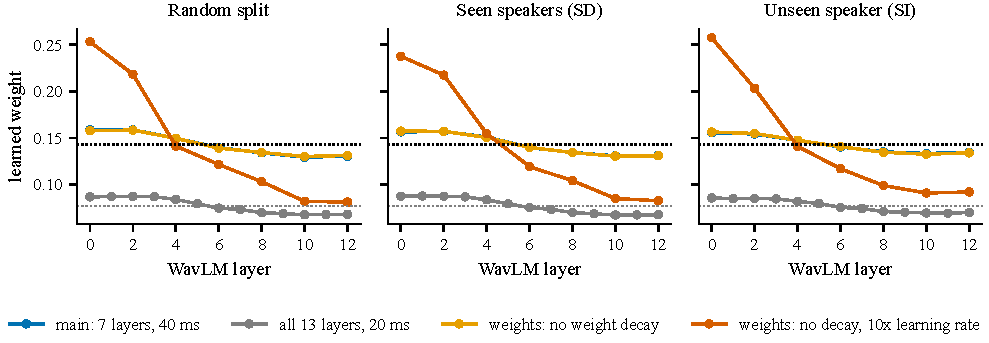
\includegraphics[width=\linewidth]{fig_layer_weights.pdf}
\caption[Learned layer weights of the speech model]{Learned layer weights (mean over runs). Only the 10$\times$ learning-rate variant departs from uniform, and it shifts weight to the lowest layers.}\label{fig:ablation}
\end{figure}

\subsection{Is the SI gap overfitting? A pre-registered test}\label{sec:prereg}
The BiGRU fits the training speaker perfectly (100\% on held-out words of that speaker) and transfers poorly, with seed-to-seed swings of up to 19\pp{} on the same test speaker (55.6--74.7\% for test OAF).
This is overfitting to the \emph{speaker}, not to the clips.
We tested one fix and wrote the plan down \emph{before} running it, committed to git ahead of the results (\code{analysis/PREREGISTRATION\_si\_linear.md}): a low-capacity model whose every choice is fixed in advance.
It uses mean and std over time of all 7 cached WavLM layers (no layer selection; 10\,752 dims), StandardScaler, and L2 logistic regression.
$C$ is chosen by word-grouped 5-fold cross-validation on the \emph{training} speaker only, and the test speaker is used once.
\begin{table}[H]\centering\small
\caption[Study 1: linear model on pooled features]{Pre-registered SI experiment (\code{Results/si\_linear.md}). The linear model is deterministic, so there is one run per direction; the BiGRU shows mean [min, max] over its 3 seeds.}\label{tab:prereg}
\begin{tabular}{@{}lccc@{}}\toprule
Model & Test YAF & Test OAF & mean\\\midrule
WavLM + BiGRU (Table~\ref{tab:main}) & 53.0 [51.1, 55.9] & 63.9 [55.6, 74.7] & 58.5\\
\textbf{all-layer linear} (pre-registered) & \textbf{68.4} & 63.5 & \textbf{66.0}\\\midrule
WavLM + BiGRU + speaker norm $\dagger$ & 56.3 & 56.8 & 56.5\\
\textbf{all-layer linear + speaker norm} $\dagger$ (pre-registered secondary) & \textbf{75.3} & \textbf{66.0} & \textbf{70.6}\\\bottomrule
\end{tabular}\end{table}
The first pre-registered hypothesis is supported, but not uniformly.
The linear model beats 5 of the 6 BiGRU runs (exact McNemar $p\le0.011$ for each), by $+15.4$\pp{} for test YAF. For test OAF it ties the BiGRU's mean ($-0.4$\pp), and one lucky BiGRU seed (74.7\%) beats it.
With speaker normalisation, it beats all 6 runs of its BiGRU counterpart in both directions ($+14.1$\pp{} on average).
Its main practical gain is \emph{stability}: no seed lottery.
Two disclosures: the training-speaker CV scores 100\% for every $C$, so it cannot discriminate, and ties fall to the strongest regularisation in the grid ($C=0.001$, the first value; a code default, not written in the plan).
Within-speaker selection cannot measure transfer to a new speaker, which is the core difficulty of SI with two speakers. Because $C$ was not really selected, we checked afterwards how much it matters (post hoc, reading the test speaker; \texttt{Results/c\_sensitivity.md}). Over $C=10^{-5}$ to $10$, the mean SI accuracy stays within 63.5--68.1\% without and 66.7--72.7\% with normalisation. The registered value is not the best one, and every value beats the BiGRU, so the result is not an artefact of the tie-break.
As a sanity check, the same feature store reproduces every per-layer probe of Table~\ref{tab:probe}.

\subsection{Why does the BiGRU lose? A second pre-registered study}\label{sec:capacity}
A literature review guided the design. Benchmarks probe frozen SSL features with pooling and a linear layer~\cite{superb}, and an LSTM head on frozen wav2vec~2.0 was no better than a dense head and much less stable~\cite{pepino}. Speaker normalisation helps most on fixed-phrase corpora~\cite{pepino}.
We registered seven hypotheses before running (\code{analysis/PREREGISTRATION\_si\_capacity.md}, pushed to GitHub with a server timestamp ahead of the runs).
The design: four neural heads, 10 seeds per direction each (80 runs), the logistic-regression controls, and an \emph{inductive} normalisation variant. In the inductive variant, the test speaker's statistics come from 40 fixed calibration words only, and every model is scored on the other 160 words.
Every hyper-parameter was fixed in advance. Retrained seeds 0--2 reproduce the original runs prediction for prediction (100\% identical).
\begin{table}[H]\centering\small
\caption[Study 2: head capacity]{Head-capacity study (SI; \code{Results/capacity\_study.md}). Neural heads: mean [min, max] over 10 seeds, and the accuracy of the seed ensemble (averaged posteriors). $\dagger$ = transductive speaker normalisation.}\label{tab:capacity}
\begin{tabular}{@{}lrcccc@{}}\toprule
Head & params & Test YAF & Test OAF & mean & ensemble\\\midrule
B1 BiGRU (main) & 858k & 57.2 [44.9, 72.1] & 61.5 [53.6, 74.7] & 59.3 & 62.9\\
B2 BiGRU + norm $\dagger$ & 858k & 57.3 [43.5, 72.8] & 55.7 [48.6, 62.6] & 56.5 & 59.4\\
B3 small BiGRU + norm $\dagger$ (dim 64, dropout 0.5) & 93k & 61.4 [52.6, 70.3] & 60.3 [52.6, 70.9] & 60.9 & 66.3\\
B4 attentive stats pooling + norm $\dagger$ (no recurrence) & 430k & 58.2 [43.0, 73.5] & 55.6 [51.1, 64.0] & 56.9 & 56.9\\\midrule
L1 logistic regression, mean+std & 75k & 68.4 & 63.5 & 66.0 & --\\
L1n same + norm $\dagger$ & 75k & 75.3 & 66.0 & 70.6 & --\\
L2n mean only + norm $\dagger$ & 38k & 73.1 & 62.3 & 67.7 & --\\\midrule
A-B2 = B2 + speed augmentation (Sec.~\ref{sec:augment}) & 858k & 54.5 [45.0, 63.9] & 59.4 [53.5, 65.3] & 56.9 & 57.4\\
A-L1n = L1n + speed augmentation (Sec.~\ref{sec:augment}) & 75k & \textbf{76.4} & \textbf{67.7} & \textbf{72.0} & --\\\bottomrule
\end{tabular}\end{table}
The pre-registered test is a word-cluster bootstrap (200 test words, 10\,000 resamples) with a $\pm$2\,pp equivalence band. It holds the 10 trained seeds fixed, so it measures uncertainty over test words only.
We therefore add a \textbf{post-hoc} bootstrap over words \emph{and} seeds, which also includes training noise; both are in \code{capacity\_study.md}. Outcomes, with the post-hoc 95\% CI per direction:
\begin{itemize}\setlength\itemsep{1pt}
\item \textbf{H2, robust:} the logistic regression beats the BiGRU on identical normalised inputs by +18.0 and +10.3\pp{} ([11.6, 24.7] and [7.0, 13.6]). Under one training speaker, the linear probe is clearly the better head.
\item \textbf{H3, consistent but not robust:} the small BiGRU beats the large one by +4.2 and +4.5\pp{} and halves the seed spread in one direction. Once seed noise is included, the CIs ([$-2.3$, 11.3], [$-0.9$, 9.9]) include zero.
\item \textbf{H4, refuted:} dropping recurrence does not help. Attentive statistics pooling is \emph{worse} than the small BiGRU ($-3.2$, $-4.7$\pp; robust in one direction). B4 is also no better than the full BiGRU on the same inputs (56.9 vs.\ 56.5\%). B4 differs from B3 in both recurrence and size (4.6$\times$ the parameters), so the design cannot separate the two. The pattern fits capacity mattering more than recurrence, but does not prove it.
\item \textbf{H1, refuted:} speaker normalisation does \emph{not} help the BiGRU ($+0.1$\pp; $-5.7$\pp, CI [$-10.3$, $-1.7$]), although it helps the linear probe in both directions. The BiGRU's deficit is therefore not just speaker shift in the input statistics.
\item \textbf{H5, supported:} averaging the 10 seeds' posteriors gains +4.8 / +1.1\pp{} for B2, and more for B3 (66.3\% mean).
\item \textbf{H6, supported:} normalisation statistics from 40 calibration words are within 0.6\pp{} of the transductive ones, for the probe and for the BiGRU. Normalisation therefore needs only a short unlabelled enrolment sample of a new speaker, not their whole test set.
\item \textbf{H7, supported:} the std statistics matter. Mean-only pooling loses 2.1 and 3.7\pp.
\end{itemize}
H1 was only partly blind: 3 of its 10 seeds were already known.
Before the runs, a 2-epoch smoke test of B3 and B4 on one fold checked the code; it informed no choice.
\textbf{Conclusion.} With one training speaker, the best-justified speech model is a low-capacity, pooled, linear head on frozen WavLM with speaker normalisation. The normalisation can be computed from a 40-word enrolment sample.
We keep the BiGRU as the assignment's temporal model, but report that it overfits the training speaker, that shrinking it helps a little, and that no temporal head matched the linear probe here.

\subsection{Does augmentation help? A third pre-registered study}\label{sec:augment}
If the BiGRU overfits its one training speaker, showing it more ``voices'' of that speaker might help.
Pre-registration~2 had already announced this test, and its details were pushed to GitHub before the run (\code{analysis/PREREGISTRATION\_si\_augmentation.md}).
Every training clip is speed-perturbed at 0.9 and 1.1 (tempo and pitch change together, as in Kaldi's \texttt{speed}), WavLM features are re-extracted, and each perturbed copy is normalised as its own pseudo-speaker. Validation and test use the original audio only.
The primary test, now registered in advance, is the bootstrap over words \emph{and} seeds (\code{Results/augmentation\_study.md}; Table~\ref{tab:capacity}, last two rows).
\begin{itemize}\setlength\itemsep{1pt}
\item \textbf{HA1, not supported:} augmentation does not reliably help the BiGRU ($-2.8$ / $+3.7$\pp; CIs [$-9.6$, 3.8], [$-1.0$, 7.7]). It does make it more stable: the seed SD falls from 10.7 to 5.8 and from 5.3 to 3.5\pp.
\item \textbf{HA2, supported:} it does not hurt the linear head; it helps slightly in both directions (+1.1, +1.7\pp; CIs [0.6, 1.6], [1.0, 2.5]).
\item \textbf{HA3, not supported:} the registered prediction that it helps the BiGRU more than the linear head fails (difference $-3.9$ / $+1.9$\pp, both CIs include zero).
\end{itemize}
The BiGRU stays 20.8 and 6.6\pp{} behind the linear head. The augmented linear model (72.0\%~$\dagger$) is the best SI result with WavLM-Base+; Sec.~\ref{sec:backbones} tests larger encoders. Augmentation therefore stabilises the BiGRU without fixing its transfer, which again points to the head rather than to the amount of training variation.

\subsection{Is the encoder the bottleneck? A fourth pre-registered study}\label{sec:backbones}
Studies 1--3 fixed the head; study~4 asks whether a stronger frozen encoder transfers better (\code{analysis/PREREGISTRATION\_si\_backbones.md}, pushed before the run).
The candidates are encoders whose authors document training data that excludes TESS: WavLM-Large~\cite{wavlm} and HuBERT-Large~\cite{hubert} (audiobooks; WavLM also podcasts and parliament speech; no labels), and emotion2vec base~\cite{emotion2vec} (262\,h of five emotion corpora, trained \emph{without} emotion labels).
Each is used with the unchanged A-L1n recipe (C fixed at 0.001, no re-tuning).
The primary model was fixed in advance as the equal-weight ensemble (ENS) of the four encoders including WavLM-Base+, so that no encoder is chosen on the test speaker.
Excluded by rule: every emotion2vec+ model, because the seed model is fine-tuned with labels on EmoBox~\cite{emobox}, which contains TESS. The larger emotion2vec+ models use undisclosed pseudo-labelled data.
All registered audits pass: each (speaker, word) pair occurs once in every emotion, so word identity carries no label information; no clip or speaker is shared between training and test; and A-L1n(B), recomputed in the job, gives 100\% identical predictions to study~3.
\begin{table}[H]\centering\small
\caption[Study 4: frozen speech encoders]{Encoder study (SI, A-L1n recipe, $\dagger$; \code{Results/backbone\_study.md}). $\Delta$ = difference from WavLM-Base+ with the 95\% word-bootstrap CI. LC rows are a leakage control, never a candidate.}\label{tab:backbones}
\begin{tabular}{@{}lccccc@{}}\toprule
Encoder & Test YAF & Test OAF & mean & $\Delta$ test YAF & $\Delta$ test OAF\\\midrule
B: WavLM-Base+ (= A-L1n) & 76.4 & 67.7 & 72.0 & -- & --\\
WL: WavLM-Large & \textbf{80.0} & \textbf{71.4} & \textbf{75.7} & +3.6 [2.6, 4.7] & +3.6 [2.6, 4.6]\\
HL: HuBERT-Large & 75.8 & 66.6 & 71.2 & $-0.6$ [$-1.8$, 0.6] & $-1.1$ [$-2.0$, $-0.1$]\\
E: emotion2vec base & 68.3 & 67.8 & 68.0 & $-8.1$ [$-10.1$, $-6.1$] & +0.1 [$-1.8$, 1.9]\\
ENS (primary, B+WL+HL+E) & 77.8 & 68.1 & 72.9 & +1.4 [0.4, 2.4] & +0.4 [$-0.4$, 1.1]\\\midrule
LC: emotion2vec+ seed, our recipe & 100.0 & 99.8 & 99.9 & & \\
LC: its own head, no training & 85.7 & 85.7 & 85.7 & & \\\bottomrule
\end{tabular}\end{table}
\begin{itemize}\setlength\itemsep{1pt}
\item \textbf{HB1 (primary), not supported:} the ensemble beats WavLM-Base+ in one direction only (+1.4\pp, CI [0.4, 2.4]; +0.4\pp, CI [$-0.4$, 1.1]).
\item \textbf{HB2:} WavLM-Large is better in both directions by the same margin (+3.6\pp, Holm $p<0.001$). HuBERT-Large is equivalent within $\pm$2\pp. emotion2vec base is 8.1\pp{} worse in one direction and equal in the other.
\item \textbf{HB3, supported:} the ensemble with 40-word enrolment statistics is within 0.1\pp{} of the transductive one.
\end{itemize}
By the registered reporting rule, the ensemble does not become the best system. The rule did not anticipate one member beating the reference in both directions. We report A-L1n with WavLM-Large (75.7\%~$\dagger$; 80.1 / 71.2\% with 40-word enrolment, on the other 160 words) as the best clean speech model, and state openly that it is the best of three tested encoders; the Holm correction covers that choice within this study (not the sequence of studies; Sec.~\ref{sec:concl}). A post-hoc sweep over C (diagnostic only) keeps it between 74.5 and 76.1\%, so the gain does not depend on a lucky C.
\textbf{Leakage control.} emotion2vec+ seed, whose training data contains TESS, scores 99.9\% on the ``unseen'' speaker with our recipe. With its own classifier and no training on our side it scores 85.7\%: a sample of 112 clips (\code{Results/lc\_zero\_shot\_check.md}) shows every clip of the six shared emotions correct, and every pleasant-surprise clip labelled ``other'', never ``surprised''. This pattern is consistent with training on TESS's own labels (we did not verify EmoBox's label mapping). Unseen-speaker scores on TESS are therefore meaningful only if the encoder's training data is documented to exclude TESS.

\subsection{Can clean levers push further? A fifth pre-registered study}\label{sec:final}
Study~5 (\code{analysis/PREREGISTRATION\_si\_final.md}, pushed before the run) tests three levers on top of A-L1n with WavLM-Large. Each is allowed by the assignment and was motivated before any test:
\begin{itemize}\setlength\itemsep{1pt}
\item \textbf{W3:} the frozen encoder of Whisper-large-v3~\cite{whisper}. It is ahead of WavLM-Large on most EmoBox cross-corpus pairs~\cite{emobox}. It was trained only to transcribe, so it cannot have learned TESS's emotion labels even if TESS audio was in its web data: every TESS transcript is ``Say the word \dots''.
\item \textbf{P:} four pitch-shifted copies of each training clip ($\pm$2 and $\pm$4 semitones, tempo kept), aimed at the age difference between the two voices (26 vs.\ 64 years).
\item \textbf{S:} self-training on the unseen speaker's unlabelled clips. In three rounds, the 25, 50 and then 75\% most confident clips are pseudo-labelled, with no class quota and no class prior.
\end{itemize}
The primary model, FINAL, applies S to the equal-weight ensemble of the P-augmented WavLM-Large and Whisper models.
Excluded by rule: other labelled corpora; encoders trained with emotion labels; and any use of TESS's design at test time (each word in all seven emotions, equal class sizes).
All audits pass. In the inductive variant no scored clip is ever pseudo-labelled (D5), and the reference model, with its features re-extracted, gives 100\% identical predictions to study~4 (C1).
\begin{table}[H]\centering\small
\caption[Study 5: Whisper encoder, pitch augmentation and self-training]{Study 5 (SI, $\dagger$; \code{Results/final\_study.md}). $\Delta$ = difference from the reference R, with the 95\% word-bootstrap CI.}\label{tab:final}
\begin{tabular}{@{}lccccc@{}}\toprule
Model & Test YAF & Test OAF & mean & $\Delta$ test YAF & $\Delta$ test OAF\\\midrule
R: A-L1n, WavLM-Large (study 4) & 80.0 & 71.4 & \textbf{75.7} & -- & --\\
W3: A-L1n, Whisper-large-v3 & 78.0 & 73.9 & 75.9 & $-2.0$ [$-2.9$, $-1.2$] & +2.5 [1.4, 3.6]\\
P: R + pitch copies & 77.3 & 71.6 & 74.5 & $-2.7$ [$-3.5$, $-2.0$] & +0.3 [$-0.6$, 1.2]\\
S: R + self-training & 82.4 & 63.0 & 72.7 & +2.4 [1.6, 3.1] & $-8.4$ [$-9.6$, $-7.1$]\\
ENS2: P on both encoders (descriptive) & 77.8 & 73.6 & 75.7 & & \\
FINAL (primary): S on ENS2 & 75.6 & 71.6 & 73.6 & $-4.4$ [$-5.3$, $-3.5$] & +0.2 [$-0.7$, 1.1]\\\bottomrule
\end{tabular}\end{table}
\begin{itemize}\setlength\itemsep{1pt}
\item \textbf{H1 (primary), not supported:} FINAL is 4.4\pp{} worse for test YAF and equal for test OAF.
\item \textbf{H2:} no lever helps in both directions. Whisper and self-training each help in one direction and hurt in the other. Pitch augmentation hurts one direction and is neutral in the other. Every non-zero difference survives the Holm correction ($p<0.001$).
\item \textbf{H3, supported:} FINAL with a 40-word enrolment is within 0.1\pp{} of the transductive version.
\end{itemize}
By the registered rule, A-L1n with WavLM-Large (75.7\%~$\dagger$) remains the best system. Whisper's 75.9\% mean is not promoted: its gain and loss split by direction, and the rule forbids choosing on the test speaker.
A post-hoc diagnostic (\code{Results/final\_selftrain\_diagnostic.csv}) explains the failure of self-training. The pseudo-labels of the first two rounds are 93--100\% correct. In the third round, which labels 75\% of the pool, accuracy drops to 79--94\%, and lowest (79--82\%) for test OAF, where self-training hurts most: the refitted model learns its own errors.
Across studies 1--5, no clean lever beyond the larger encoder improved both directions.

% =====================================================================
\section{Analysis (C)}\label{sec:analysis}
\subsection{Which emotions are easiest and hardest?}\label{sec:easy}
\begin{table}[H]\centering\small
\caption[Per-class F1 on the unseen speaker]{Per-class F1 (\%) under SI, mean over 6 runs. Under RAND/SD every class is $\ge98.8$ for all audio models.}\label{tab:f1}
\begin{tabular}{@{}lccccccc@{}}\toprule
Model & Angry & Disgust & Fear & Happy & Neutral & Pl.\ surprise & Sad\\\midrule
Speech log-Mel & 20.7 & 51.0 & 30.9 & 0.6 & 83.8 & 13.6 & 52.7\\
Speech WavLM & 15.0 & 74.9 & 66.1 & 6.6 & 89.9 & 36.6 & 84.4\\
Text, Whisper ASR & 16.7 & 12.1 & 18.6 & 1.1 & 25.7 & 35.6 & 12.2\\
Fusion GMU (GT) & 23.1 & 59.2 & 70.1 & 6.9 & 90.7 & 24.6 & \textbf{91.8}\\
Fusion cross-attn (GT) & 24.6 & 69.6 & \textbf{77.1} & 6.3 & \textbf{95.1} & \textbf{43.9} & 82.5\\\bottomrule
\end{tabular}\end{table}

\begin{figure}[H]\centering
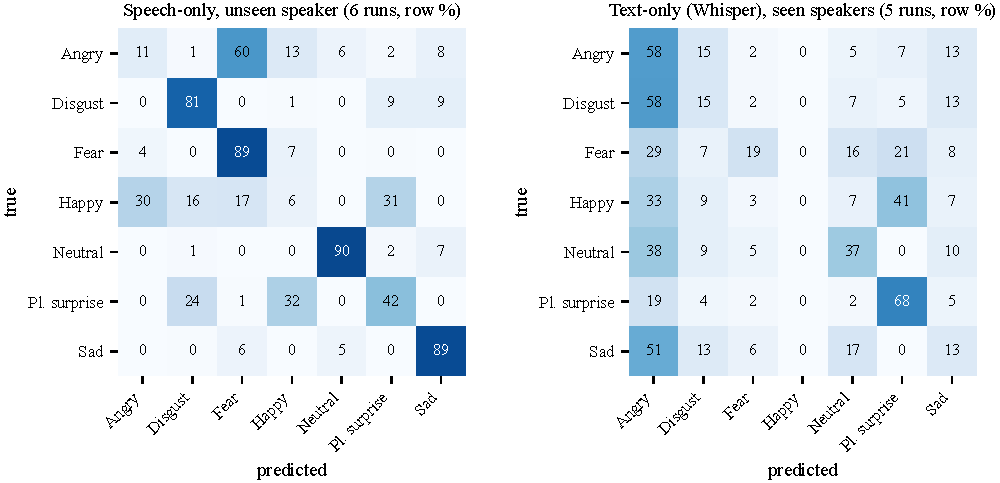
\includegraphics[width=\linewidth]{fig_confusions.pdf}
\caption[Confusion matrices of the speech and text models]{Row-normalised confusion matrices. Left: speech WavLM, SI (6 runs). Right: text model on Whisper transcripts, SD. It can only separate classes whose ASR punctuation differs, and pleasant surprise is the most distinctive.}\label{fig:conf}
\end{figure}

\textbf{Easiest: neutral, sad, fear} (SI F1 90--95, 82--92 and 66--77 for the WavLM-based models).
They sit at the extremes of the arousal axis.
Neutral and sad are low-arousal: low, flat F0 and low energy. Sad is also among the longest (2.36\,s on average; only disgust is longer, at 2.39\,s).
Fear has its own high, tense, short profile (the shortest class, 1.60\,s).
These are \emph{global} prosodic properties that change little between speakers once the speaker's own level is accounted for.
\textbf{Hardest: happy (F1 $\le$7) and angry (15--25)}, then pleasant surprise.
They are all high-arousal and differ mainly in \emph{valence}, which acoustics encode weakly.
The confusion matrix (Fig.~\ref{fig:conf}) shows the structure: happy is split between angry (30\%), pleasant surprise (31\%), fear and disgust, and angry is mostly called fear (60\%).
How these classes are realised depends on the speaker: the two transfer directions differ by up to 13\pp{} for the same model.
None of this shows under RAND/SD (every class $\ge$98.8), which is another sign that those protocols mostly test recognition of a known speaker's style.

\subsection{When does fusion help?}\label{sec:whenfusion}
\textbf{Ground-truth text cannot help, and the model learns that only partly.}
Every word appears once per emotion and speaker, so $I(\text{text};y)=0$, and the probes, the zero-shot model and the trained text model all confirm it.
The GMU gate puts most weight on speech (mean $z=0.84$ in SI; Fig.~\ref{fig:gate}), but not all of it.
The remaining weight on text ($1-z\approx0.16$ on average) injects word-identity variance that is useless for the label.
This is consistent with GMU-GT being slightly (n.s.) \emph{below} speech-only under SI ($-1.7$\pp).
Concatenation and cross-attention are not hurt and even gain (+1.6, +4.9\pp, n.s.).
A plausible mechanism: text is independent of the \emph{label} but not of the \emph{acoustics}.
Knowing which word was said lets cross-attention condition the speech pooling on lexical content and partly factor phonetic variation out of the prosodic evidence.
With six runs we cannot confirm this.

\begin{table}[H]\centering\small
\caption[Punctuation in Whisper transcripts by emotion]{What Whisper-small writes for each emotion (\% of clips). The trained text model can only read these marks; the target word is recognised for 84--92\% of clips regardless of emotion.}\label{tab:asr}
\begin{tabular}{@{}lccccccc@{}}\toprule
& Angry & Disgust & Fear & Happy & Neutral & Pl.\ surprise & Sad\\\midrule
ends with ``!'' & 9.2 & 4.5 & 32.0 & 42.8 & 0.0 & \textbf{72.2} & 0.0\\
ends with ``.'' & 90.8 & 95.5 & 65.0 & 57.2 & 87.2 & 27.5 & \textbf{99.5}\\
ends with ``?'' & 0 & 0 & 2.8 & 0 & 0.5 & 0.2 & 0\\
exact carrier sentence & 85.0 & 84.0 & 59.0 & 79.8 & 63.5 & 86.2 & 70.8\\\bottomrule
\end{tabular}\end{table}

\textbf{ASR transcripts carry prosody, through punctuation.}
Whisper's punctuation and casing are predicted from the audio, so excited speech gets an exclamation mark and a long pause gets a comma (\emph{``Say the word, bar.''} is typical of neutral and sad).
This is why the Whisper text model reaches 2.1$\times$ chance while the emotion-tuned zero-shot model, which reads the \emph{words}, stays at chance.
The text model's best class is pleasant surprise (F1 56 in SD), exactly the class with the most ``!''.
However, this text signal is a lossy, quantised copy of information the speech branch already has, so it adds little \emph{on average} (GMU-Whisper vs.\ GMU-GT: $+0.4$\pp, $p=0.91$).

\begin{figure}[H]\centering
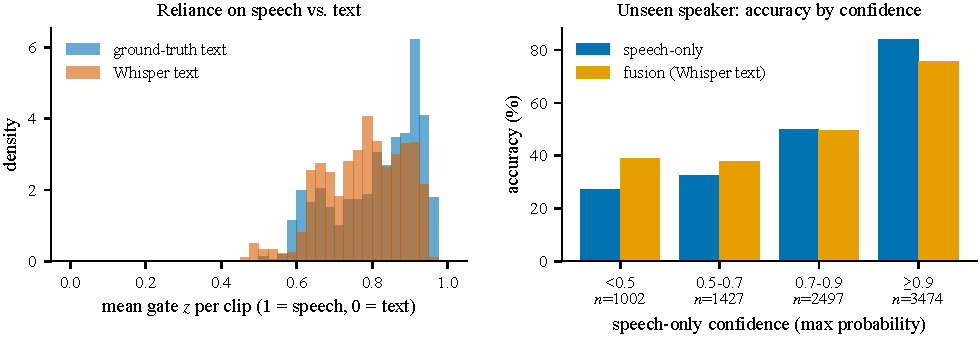
\includegraphics[width=\linewidth]{fig_fusion.pdf}
\caption[Fusion gate and accuracy by speech confidence]{Left: distribution of the mean GMU gate per test clip (1 = speech). Right: SI accuracy of speech-only vs.\ GMU fusion (Whisper), binned by the speech-only model's confidence on the same clip.}\label{fig:gate}
\end{figure}

\textbf{Fusion helps when the speech evidence is weak.}
Binning SI test clips by the speech-only model's confidence (Fig.~\ref{fig:gate}, right) shows a clear crossover:

\begin{center}\small
\begin{tabular}{@{}lcccc@{}}\toprule
speech confidence & $<$0.5 & 0.5--0.7 & 0.7--0.9 & $\ge$0.9\\\midrule
clips & 1002 & 1427 & 2497 & 3474\\
speech-only acc. & 27.3 & 32.6 & 50.1 & 84.1\\
fusion (Whisper) acc. & 39.1 & 37.8 & 49.6 & 75.7\\
$\Delta$ & \textbf{+11.8} & \textbf{+5.3} & $-0.5$ & $-8.4$\\\bottomrule
\end{tabular}\end{center}

The same pattern holds, more weakly, for ground-truth text (+4.9 / +1.1 / $-3.2$ / $-3.7$).

\textbf{But part of this crossover is a statistical artefact.} Binning clips by model A's confidence selects clips where A happens to be wrong, so \emph{any} second model looks better in A's low-confidence bins and worse in its high ones (regression to the mean).
We measure the artefact directly by replacing fusion with a second \emph{speech-only} model (another seed, same direction; \code{robustness\_checks.md}).
It ``gains'' +6.1 / +3.9 / +1.4 / $-4.4$\pp{} across the four bins, with no new information at all.
Net of this control, Whisper-text fusion gains \textbf{+5.7}\pp{} for clips with speech confidence $<$0.5 and +1.4\pp{} at 0.5--0.7, and loses 1.9--4.0\pp{} at higher confidence.
Ground-truth-text fusion shows \emph{no} net gain in any bin ($-4.6$ to $+0.7$\pp).
So the defensible claim is narrower: text that carries prosodic traces (ASR punctuation) adds a little where speech is ambiguous, and label-independent text does not.
Where speech is confident, fusion hurts, and the gate stays at $\approx0.77$ regardless of confidence (Whisper model; it was learned on the training speaker, where speech is almost always right).
A confidence-aware or per-clip-calibrated gate is the obvious next step.
Under noise (\S\ref{sec:noise}), where speech degrades, the fusion models did \emph{not} gain meaningfully over speech-only, because the noisy-ASR transcripts lose their punctuation cue as well (see the table in that section).

\subsection{Error analysis: five systematic failure cases}\label{sec:errors}
695 of 2800 SI test clips are misclassified by the gated fusion model in \emph{every} seed. Most of these errors are systematic, not random.
The most frequent confusions (true class predicted as another) are happy as angry (123), pleasant surprise as happy (118), angry as fear (91) and happy as pleasant surprise (75).
For each case below, we compare the clip's prosody with \emph{the same speaker's} average for the true and predicted classes (\code{Results/error\_analysis.md}):

\begin{figure}[H]\centering
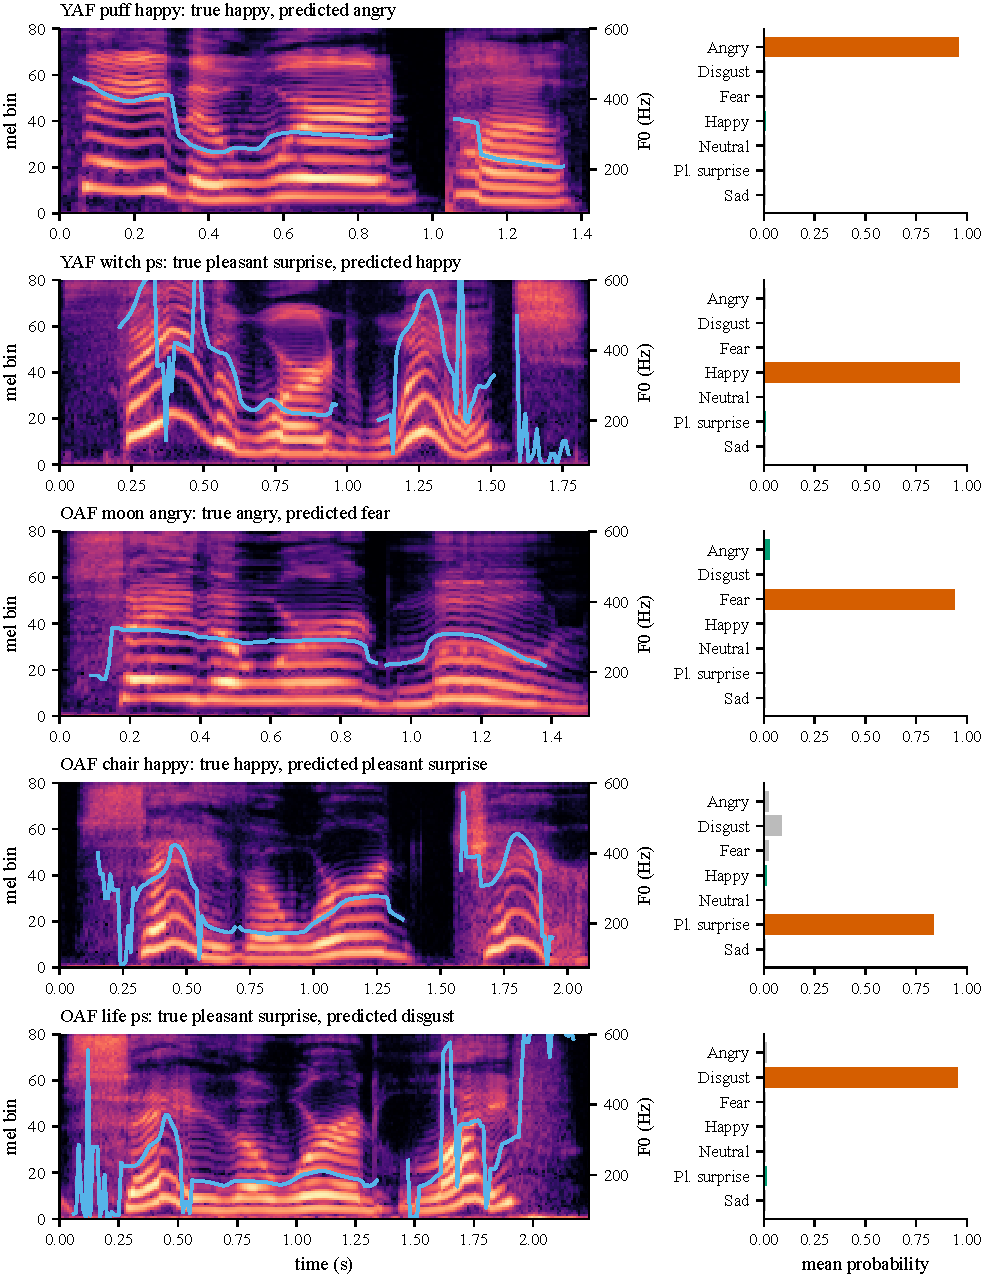
\includegraphics[width=\linewidth]{fig_error_cases.pdf}
\caption[Five systematic failure cases]{Five clips misclassified by GMU fusion in all SI seeds: log-Mel spectrogram with F0 (left) and mean posterior (right; orange = predicted, green = true).}\label{fig:errors}
\end{figure}
\begin{enumerate}\setlength\itemsep{1pt}
\item \textbf{YAF\_puff\_happy, predicted angry (p = 0.96).} F0 median (294\,Hz) and energy ($-16.2$\,dB) are close to YAF's \emph{happy} means (280\,Hz, $-15.9$\,dB) and far from angry (237\,Hz, $-18.0$\,dB); the F0 range fits both classes (218 vs.\ 202/216\,Hz), and the duration is shorter than either (1.42\,s). Its own prosody points to the correct class rather than the predicted one, so this is a pure \emph{cross-speaker mapping} error. The region the OAF-trained model calls ``angry'' covers YAF's happy, the most frequent confusion overall (123 clips).
\item \textbf{YAF\_witch\_ps, predicted happy (0.96).} Median F0 (296\,Hz) and energy are closer to happy than to pleasant surprise. The very wide F0 range (523\,Hz) is partly pitch-tracker octave jumps on a creaky ending (Fig.~\ref{fig:errors}). Both classes are high-arousal with rising contours, and what separates them is valence, which acoustics encode weakly.
\item \textbf{OAF\_moon\_angry, predicted fear (0.94).} This is the one case where global prosody clearly favours the prediction. The F0 median (290\,Hz) equals OAF-fear's (291\,Hz vs.\ 268\,Hz for angry), the range is compressed (99\,Hz vs.\ 209\,Hz angry, 148\,Hz fear) and the contour is flat and tense. Prosodically the clip \emph{is} the speaker's fear profile, so the label itself is arguably ambiguous.
\item \textbf{OAF\_chair\_happy, predicted pleasant surprise (0.84).} The utterance-level functionals do not favour surprise (F0 range 265\,Hz, smaller than both class means, and lower energy). But the target word carries a large rise-fall in F0 (peak $\approx$400\,Hz at 1.8\,s), the archetypal surprise contour. The model follows this \emph{local} cue on the final word, as attention pooling allows.
\item \textbf{OAF\_life\_ps, predicted disgust (0.95).} Median F0 (201\,Hz) and energy match OAF-ps (203\,Hz), not disgust (183\,Hz). Only the long duration (2.24\,s, close to disgust's 2.34\,s) and the slow, low middle section point to disgust. The surprise rise is confined to the last word and is irregular (voicing breaks), so the model weights the slow delivery more heavily than the final rise.
\end{enumerate}
\textbf{Common pattern.} Only one of the five errors (case 3) is explained by the clip's global prosody resembling the predicted class.
In the others, the speaker-relative functionals favour the \emph{true} class or are mixed, and the error comes from (a) the class regions learned on the other speaker not lining up with this speaker's (cases 1 and 2, matching the displaced clusters in Fig.~\ref{fig:tsne}), or (b) a single salient local cue (a final rise or a slow segment) overriding the rest (cases 4 and 5).
The fix suggested by (a) is speaker adaptation or normalisation; by (b), richer pooling over several cues.
The confidences are also \emph{high} (0.84--0.96): errors are confident, not borderline (see calibration below).

\subsection{Separability of the temporal, contextual and fusion blocks}\label{sec:separability}
\begin{figure}[H]\centering
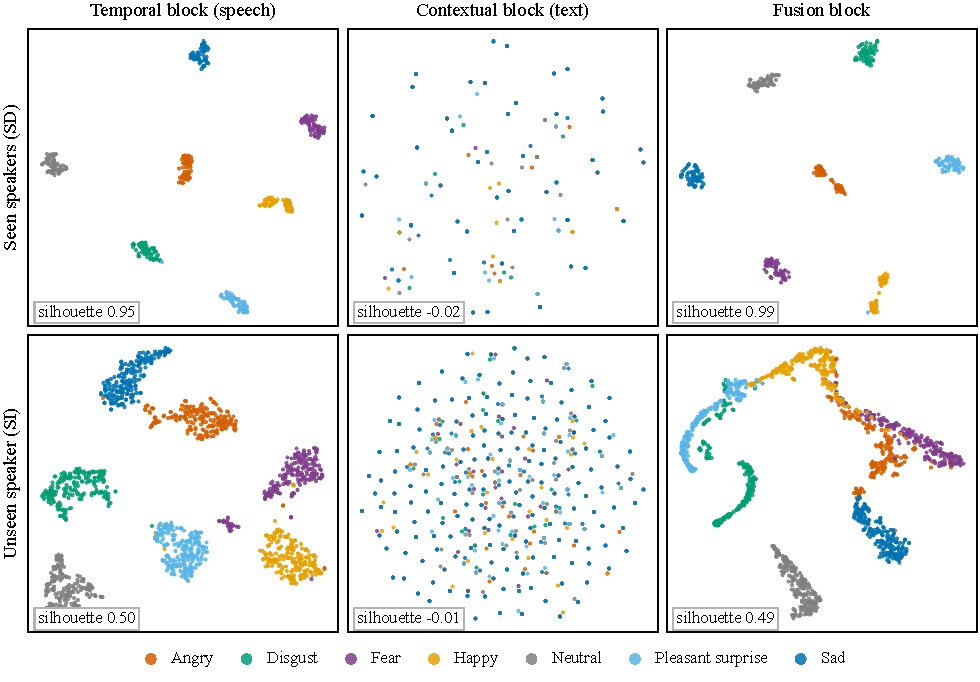
\includegraphics[width=\linewidth]{fig_tsne.pdf}
\caption[Separability of the temporal, contextual and fusion blocks]{t-SNE~\cite{tsne} of the test-set outputs of the three required blocks (attention-pooled 256-d embeddings), coloured by true emotion. Top: seen speakers (SD, seed 0). Bottom: unseen speaker (SI, trained on OAF, tested on YAF). Panel silhouettes (cosine, in the original 256-d space) are for the run shown; the table below gives means over all runs. The text panels show few distinct points because every clip of the same word has the same transcript, hence the same embedding. The speaker-normalised and Whisper-transcript variants are in the table below and \code{Results/plots/tsne\_blocks\_*.png}.}\label{fig:tsne}
\end{figure}

\begin{center}\small
\begin{tabular}{@{}lcccccc@{}}\toprule
silhouette & \begin{tabular}[c]{@{}c@{}}temporal\\speech\end{tabular} & \begin{tabular}[c]{@{}c@{}}temporal\\+spk-norm\end{tabular} & \begin{tabular}[c]{@{}c@{}}contextual\\GT text\end{tabular} & \begin{tabular}[c]{@{}c@{}}contextual\\Whisper\end{tabular} & \begin{tabular}[c]{@{}c@{}}fusion\\GMU-GT\end{tabular} & \begin{tabular}[c]{@{}c@{}}fusion\\GMU-Whisper\end{tabular}\\\midrule
SD & 0.96 $\pm$ 0.01 & 0.97 $\pm$ 0.01 & $-0.02$ $\pm$ 0.00 & $-0.22$ $\pm$ 0.05 & 0.99 $\pm$ 0.01 & 0.95 $\pm$ 0.01\\
SI & 0.57 $\pm$ 0.04 & 0.57 $\pm$ 0.06 & $-0.01$ $\pm$ 0.00 & $-0.22$ $\pm$ 0.07 & 0.54 $\pm$ 0.08 & 0.47 $\pm$ 0.07\\\bottomrule
\end{tabular}\end{center}

Silhouettes are mean $\pm$ std over all test runs (5 SD, 6 SI; \code{Results/silhouette\_all\_runs.csv}); Fig.~\ref{fig:tsne} shows one run of each protocol.
\textbf{Temporal block (speech).} Under SD, the seven emotions form tight, well-separated clusters (silhouette 0.96).
Under SI, the unseen speaker's emotions still form largely separate clusters (0.57; Fig.~\ref{fig:tsne}, bottom left), yet the mean accuracy is only 58.5\%.
The representation therefore separates much of the new speaker's emotions. What fails is that the clusters are \emph{displaced} relative to the decision boundaries learned on the training speaker.
Label-free speaker normalisation leaves the silhouette unchanged (0.57), consistent with moving the new speaker's clusters rather than reshaping them; it is the linear model with this normalisation that reaches 75.3\% on test YAF (\S\ref{sec:prereg}).
\textbf{Contextual block (text).} With ground-truth text the embeddings are an unstructured cloud (silhouette $\approx$0): the text block encodes words, not emotion.
With Whisper text, groups appear, but they are groups of \emph{transcript forms} (ending in ``!'' vs.\ ``.'', comma or no comma), each mixing several emotions; hence the negative silhouette.
\textbf{Fusion block.} Under SD, fusion clusters are as tight as speech (0.99 vs.\ 0.96) and are organised by the speech geometry.
Under SI they are slightly less separated than speech alone (0.54 with ground-truth text, 0.47 with Whisper text), and the clusters stretch into elongated manifolds, consistent with the text dimensions adding word-wise variation along directions orthogonal to emotion.

\subsection{Robustness to noise and the value of speaker normalisation}\label{sec:noise}
\begin{figure}[H]\centering
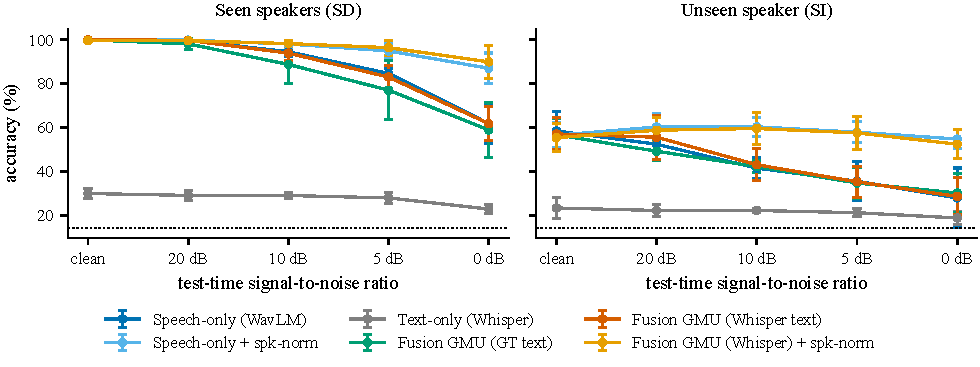
\includegraphics[width=\linewidth]{fig_noise.pdf}
\caption[Robustness to additive white noise]{Test-time additive white noise. Models are trained on clean audio; WavLM, Whisper and DistilRoBERTa features are recomputed from the noisy audio. Mean $\pm$ std over 5 (SD) / 6 (SI) runs.}\label{fig:noise}
\end{figure}
\begin{center}\small
\begin{tabular}{@{}llccccc@{}}\toprule
& Model & clean & 20\,dB & 10\,dB & 5\,dB & 0\,dB\\\midrule
SD & Speech WavLM & 99.9 & 99.7 & 94.5 & 84.6 & 61.8\\
& Speech + speaker norm $\dagger$ & 100.0 & 99.8 & 98.0 & 94.9 & \textbf{87.0}\\
& Fusion GMU (Whisper) & 100.0 & 99.7 & 93.9 & 83.0 & 61.8\\
& Fusion GMU (Whisper) + speaker norm $\dagger$ & 99.6 & 99.6 & 98.2 & 96.4 & \textbf{89.9}\\\midrule
SI & Speech WavLM & 58.5 & 52.5 & 41.6 & 35.6 & 28.0\\
& Speech + speaker norm $\dagger$ & 56.5 & \textbf{60.3} & \textbf{60.4} & 57.9 & \textbf{54.8}\\
& Fusion GMU (GT) & 56.8 & 49.3 & 42.3 & 34.8 & 30.3\\
& Fusion GMU (Whisper) + speaker norm $\dagger$ & 55.4 & 58.8 & 59.6 & 57.6 & 52.5\\
& Text only (Whisper) & 23.5 & 22.3 & 22.3 & 21.3 & 18.9\\\bottomrule
\end{tabular}\end{center}
Without normalisation, accuracy degrades steadily, and at 0\,dB the SI models are only 2$\times$ chance.
With label-free per-speaker normalisation of the WavLM features, the statistics are re-estimated on each speaker's (noisy, unlabelled) test audio, i.e.\ test-time CMVN.
The SD model then keeps 87--90\% at 0\,dB, and the SI model is essentially \emph{flat} from clean to 0\,dB (from 56.5 to 54.8\%), even slightly \emph{better} at 10--20\,dB than on clean audio.
Stationary white noise mostly shifts and scales the feature distribution, which per-speaker standardisation removes.
The same mechanism removes some of the speaker shift.
This is transductive: it needs a batch of unlabelled audio from the test speaker and condition. That is cheap in practice, but it is why we report it separately ($\dagger$) and never in the main comparison.
Text-only (Whisper) is the most \emph{stable} pipeline ($-4.6$\pp{} at 0\,dB), but only because it starts low.
Noisy ASR loses the exclamation cue (from 16.6\% of transcripts ending in ``!'' at 20\,dB to 10.6\% at 0\,dB, \code{noise\_asr\_punctuation.json}) and starts producing ``?''.
So the text branch cannot compensate for degraded speech, and fusion without normalisation degrades as fast as speech.

\textbf{Calibration.} Under RAND/SD all audio models are well calibrated (ECE about 3\%).
Under SI they are badly over-confident~\cite{guo}: the WavLM model has 78.5\% mean confidence at 58.5\% accuracy (ECE 20.9\%), and GMU fusion is worse (86--87\% confidence at 57\%, ECE 29--30\%).
Fusion adds confidence without adding accuracy.
Any deployment would need re-calibration on the target speaker (e.g.\ temperature scaling) before the confidence-based gating suggested above could work.

% =====================================================================
\section{Conclusions and limitations}\label{sec:concl}
\begin{itemize}\setlength\itemsep{1pt}
\item \textbf{Best pipeline.} Speech carries essentially all the emotion information in TESS. Among the trained neural variants, fusion matches speech-only; cross-attention's higher SI mean (63.4\% vs.\ 58.5\%) comes from one transfer direction and is not significant. Text alone is useful only through ASR punctuation (2.1$\times$ chance).
\item \textbf{The real problem is speaker shift.} The BiGRU scores 100\% on unseen words of the training speaker and 58.5\% on the unseen speaker: it overfits the speaker. Three pre-registered studies show that a low-capacity linear head transfers best (66.0\%; 70.6\% with speaker normalisation, which needs only a 40-word unlabelled enrolment sample; 72.0\% with speed augmentation added; 75.7\% with frozen WavLM-Large, the best clean result; Whisper-large-v3, pitch augmentation and self-training did not improve both directions, Sec.~\ref{sec:final}). The linear head beats the BiGRU by 10--18\pp{} on identical inputs in both directions, robust to seed noise; neither normalisation nor augmentation rescues the BiGRU. Probes, t-SNE and the normalisation results all locate the gap in a speaker-dependent \emph{displacement} of otherwise largely separable emotion clusters.
\item \textbf{Limitations.} TESS has two speakers, both female, reading one carrier phrase. SI results are therefore two transfer directions: seeds within a direction are not independent, and per-direction results are reported for every claim. Every SI interval and $p$-value describes variation over words and seeds \emph{for these two speakers}, not over speakers. Studies 2--5 were each planned after seeing the earlier studies' results on the same two test speakers: pre-registration fixes the analysis within each study, but not the sequence, so the best result (75.7\%) is likely optimistic. Among the 11 original variants, no run-level difference survives correction for multiple comparisons. The capacity study's word-level tests are conditional on these two voices: they show consistency across two speakers, not generality over speakers. Conclusions about fusion apply only to text that is label-independent by construction; datasets with semantically emotional text (e.g.\ IEMOCAP, MELD) would test the fusion design properly. The frozen encoders were not fine-tuned (by design, given about 1.2--2k training clips; untested). Encoders fine-tuned with emotion labels are excluded unless their training data is documented to exclude TESS: one that includes it scores 99.9\% on the unseen speaker (Sec.~\ref{sec:backbones}).
\item \textbf{Reproducibility.} \code{python run\_all.py} reproduces every number and figure. All runs were executed on a Kaggle T4 GPU (\code{logs/kaggle\_run\_v2.log}; ablation: \code{logs/kaggle\_run\_ablation.log}, \code{run\_all.py --ablations}). Three analysis scripts in that job computed and printed their results but crashed when saving, because \code{Results/} did not yet exist (fixed). The layer probes and the prosody baseline were re-run in a separate job (\code{logs/kaggle\_run\_analyses.log}); the re-run agrees with the printed values (prosody identical, probes within 0.05\pp). The noise study needs trained checkpoints, which the first job did not keep, so it was regenerated in its own job (\code{kaggle/make\_kernel.py noise}, \code{logs/kaggle\_run\_noise.log}), with checks registered in advance: all 66 retrained runs give 100\% identical test predictions to the original runs, all Whisper transcripts (clean and noisy) are identical, and every per-run noise accuracy matches the earlier values printed in the log to within 0.05\pp{} (\code{Results/noise\_regeneration\_check.md}). Kaggle jobs are generated by \code{kaggle/make\_kernel.py}. The pre-registered SI experiment and the robustness checks (\code{analysis/si\_linear.py}, \code{analysis/robustness\_checks.py}) run on CPU from the cached features and saved predictions; the cached WavLM store reproduces the Kaggle probe results. The capacity study ran as one Kaggle job (\code{kaggle/make\_kernel.py capacity}, \code{logs/kaggle\_run\_capacity.log}; runs in \code{runs\_capacity/}); so did the augmentation study (\code{augment}, \code{runs\_augment/}) and the encoder study (\code{backbones}, \code{logs/kaggle\_run\_backbones.log}). Study~5 extracted its features in \code{final} (\code{logs/kaggle\_run\_final\_v3\_failed.log}) and ran its analysis on the saved features in \code{final\_analysis} (\code{logs/kaggle\_run\_final\_analysis.log}). Both studies needed a second job before any test was computed: study~4's first job lacked a reference file, and study~5's analysis ran out of memory (one self-training stage peaks at 29\,GB of the 32\,GB container), so each of its stages now runs in a fresh process. Both fixes left the analysis unchanged and are recorded as amendments in the plans. \code{tests/} holds invariant tests: no speaker or word leakage, label and feature alignment, label-free normalisation, every metric recomputed from predictions. Planted bugs confirm the tests can fail. A cell-by-cell check of every table against its source file is also included. Per-run predictions, metrics, embeddings and training curves for all 224 runs (176 main, 48 ablation) are in \code{runs/}.
\end{itemize}

\begin{thebibliography}{99}\small\setlength\itemsep{0pt}\refshook
\bibitem{tess} K.~Dupuis and M.~K. Pichora-Fuller, ``Toronto Emotional Speech Set (TESS),'' University of Toronto, Psychology Department, 2010. doi:10.5683/SP2/E8H2MF.
\bibitem{wavlm} S.~Chen et al., ``WavLM: Large-scale self-supervised pre-training for full stack speech processing,'' \emph{IEEE J. Sel. Topics Signal Process.}, vol.~16, no.~6, pp.~1505--1518, 2022.
\bibitem{superb} S.-w. Yang et al., ``SUPERB: Speech processing Universal PERformance Benchmark,'' in \emph{Proc. Interspeech}, 2021, pp.~1194--1198.
\bibitem{pasad} A.~Pasad, J.-C. Chou, and K.~Livescu, ``Layer-wise analysis of a self-supervised speech representation model,'' in \emph{Proc. IEEE ASRU}, 2021.
\bibitem{whisper} A.~Radford, J.~W. Kim, T.~Xu, G.~Brockman, C.~McLeavey, and I.~Sutskever, ``Robust speech recognition via large-scale weak supervision,'' in \emph{Proc. ICML}, 2023.
\bibitem{distilbert} V.~Sanh, L.~Debut, J.~Chaumond, and T.~Wolf, ``DistilBERT, a distilled version of BERT: smaller, faster, cheaper and lighter,'' arXiv:1910.01108, 2019.
\bibitem{roberta} Y.~Liu et al., ``RoBERTa: A robustly optimized BERT pretraining approach,'' arXiv:1907.11692, 2019.
\bibitem{hartmann} J.~Hartmann, ``Emotion English DistilRoBERTa-base,'' 2022. \url{https://huggingface.co/j-hartmann/emotion-english-distilroberta-base}.
\bibitem{gru} K.~Cho, B.~van Merri\"enboer, C.~Gulcehre, D.~Bahdanau, F.~Bougares, H.~Schwenk, and Y.~Bengio, ``Learning phrase representations using RNN encoder--decoder for statistical machine translation,'' in \emph{Proc. EMNLP}, 2014.
\bibitem{bahdanau} D.~Bahdanau, K.~Cho, and Y.~Bengio, ``Neural machine translation by jointly learning to align and translate,'' in \emph{Proc. ICLR}, 2015.
\bibitem{specaugment} D.~S. Park, W.~Chan, Y.~Zhang, C.-C. Chiu, B.~Zoph, E.~D. Cubuk, and Q.~V. Le, ``SpecAugment: A simple data augmentation method for automatic speech recognition,'' in \emph{Proc. Interspeech}, 2019.
\bibitem{gmu} J.~Arevalo, T.~Solorio, M.~Montes-y-G\'omez, and F.~A. Gonz\'alez, ``Gated multimodal units for information fusion,'' in \emph{ICLR Workshop Track}, 2017.
\bibitem{moddrop} N.~Neverova, C.~Wolf, G.~Taylor, and F.~Nebout, ``ModDrop: Adaptive multi-modal gesture recognition,'' \emph{IEEE Trans. Pattern Anal. Mach. Intell.}, vol.~38, no.~8, pp.~1692--1706, 2016.
\bibitem{mult} Y.-H.~H. Tsai, S.~Bai, P.~P. Liang, J.~Z. Kolter, L.-P. Morency, and R.~Salakhutdinov, ``Multimodal Transformer for unaligned multimodal language sequences,'' in \emph{Proc. ACL}, 2019.
\bibitem{adamw} I.~Loshchilov and F.~Hutter, ``Decoupled weight decay regularization,'' in \emph{Proc. ICLR}, 2019.
\bibitem{onecycle} L.~N. Smith and N.~Topin, ``Super-convergence: Very fast training of neural networks using large learning rates,'' in \emph{Proc. SPIE}, vol.~11006, 2019.
\bibitem{labelsmooth} C.~Szegedy, V.~Vanhoucke, S.~Ioffe, J.~Shlens, and Z.~Wojna, ``Rethinking the Inception architecture for computer vision,'' in \emph{Proc. CVPR}, 2016.
\bibitem{dietterich} T.~G. Dietterich, ``Approximate statistical tests for comparing supervised classification learning algorithms,'' \emph{Neural Computation}, vol.~10, no.~7, pp.~1895--1923, 1998.
\bibitem{cmvn} O.~Viikki and K.~Laurila, ``Cepstral domain segmental feature vector normalization for noise robust speech recognition,'' \emph{Speech Communication}, vol.~25, pp.~133--147, 1998.
\bibitem{egemaps} F.~Eyben et al., ``The Geneva Minimalistic Acoustic Parameter Set (GeMAPS) for voice research and affective computing,'' \emph{IEEE Trans. Affective Computing}, vol.~7, no.~2, pp.~190--202, 2016.
\bibitem{tsne} L.~van der Maaten and G.~Hinton, ``Visualizing data using t-SNE,'' \emph{J. Mach. Learn. Res.}, vol.~9, pp.~2579--2605, 2008.
\bibitem{pepino} L.~Pepino, P.~Riera, and L.~Ferrer, ``Emotion recognition from speech using wav2vec 2.0 embeddings,'' in \emph{Proc. Interspeech}, 2021, pp.~3400--3404.
\bibitem{hubert} W.-N. Hsu, B.~Bolte, Y.-H.~H. Tsai, K.~Lakhotia, R.~Salakhutdinov, and A.~Mohamed, ``HuBERT: Self-supervised speech representation learning by masked prediction of hidden units,'' \emph{IEEE/ACM Trans. Audio, Speech, Lang. Process.}, vol.~29, pp.~3451--3460, 2021.
\bibitem{emotion2vec} Z.~Ma et al., ``emotion2vec: Self-supervised pre-training for speech emotion representation,'' in \emph{Findings of ACL}, 2024.
\bibitem{emobox} Z.~Ma et al., ``EmoBox: Multilingual multi-corpus speech emotion recognition toolkit and benchmark,'' in \emph{Proc. Interspeech}, 2024.
\bibitem{guo} C.~Guo, G.~Pleiss, Y.~Sun, and K.~Q. Weinberger, ``On calibration of modern neural networks,'' in \emph{Proc. ICML}, 2017.
\end{thebibliography}


\end{document}
